%%%%%%%%%%%%%%%%%%%%%%%%%%%%%%%%%%%%%%%%%
% University/School Laboratory Report
% LaTeX Template
% Version 3.1 (25/3/14)
%
% This template has been downloaded from:
% http://www.LaTeXTemplates.com
%
% Original author:
% Linux and Unix Users Group at Virginia Tech Wiki
% (https://vtluug.org/wiki/Example_LaTeX_chem_lab_report)
%
% License:
% CC BY-NC-SA 3.0 (http://creativecommons.org/licenses/by-nc-sa/3.0/)
%
%%%%%%%%%%%%%%%%%%%%%%%%%%%%%%%%%%%%%%%%%

%----------------------------------------------------------------------------------------
%	PACKAGES AND DOCUMENT CONFIGURATIONS
%----------------------------------------------------------------------------------------

\documentclass{article}

\usepackage{graphicx} % Required for the inclusion of images
\usepackage{natbib} % Required to change bibliography style to APA
\usepackage{amsmath} % Required for some math elements
\usepackage{mathtools}
\usepackage[export]{adjustbox}
\usepackage{subcaption}
\usepackage{float}
\usepackage{listings}
\usepackage[margin=1.0in]{geometry}
\usepackage{minted}

\DeclarePairedDelimiter{\abs}{\lvert}{\rvert}
\setlength\parindent{0pt} % Removes all indentation from paragraphs

\renewcommand{\labelenumi}{\alph{enumi}.} % Make numbering in the enumerate environment by letter rather than number (e.g. section 6)

%\usepackage{times} % Uncomment to use the Times New Roman font

%----------------------------------------------------------------------------------------
%	DOCUMENT INFORMATION
%----------------------------------------------------------------------------------------

\title{ECE 637 Digital Image Processing Laboratory: \\ Image Halftoning} % Title

\author{Yang \textsc{Wang}} % Author name

\date{\today} % Date for the report

\begin{document}

\maketitle % Insert the title, author and date

%----------------------------------------------------------------------------------------
%	SECTION 1
%----------------------------------------------------------------------------------------

\section{Introduction}

Nothing due for report.

%----------------------------------------------------------------------------------------
%	SECTION 2
%----------------------------------------------------------------------------------------

\section{Image Fidelity Metrics}

Nothing due for report.

%----------------------------------------------------------------------------------------
%	SECTION 3
%----------------------------------------------------------------------------------------

\section{Thresholding and Random Noise Binarization}

In this section, the technique of using thresholding to convert a grayscale
image to a binary image is explored. Using a single threshold value, a grayscale
image is converted to a binary image associated with root mean square error
(RMSE) and fidelity value. These values are also calculated.

\subsection{Original Image vs. Threshold Image}
	\begin{figure}[h]
		\begin{subfigure}{0.5\textwidth}
			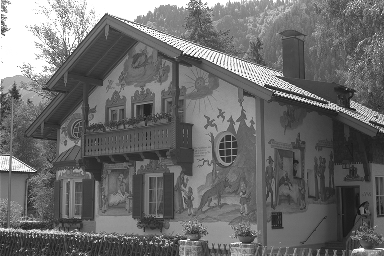
\includegraphics[width=0.9\textwidth]{house.png}
			\caption{Original house.tif}
		\end{subfigure}
		\begin{subfigure}{0.5\textwidth}
			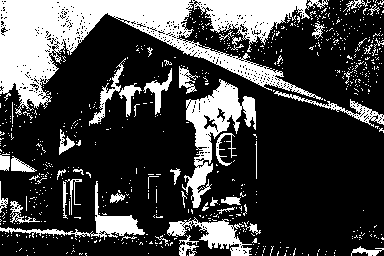
\includegraphics[width=0.9\textwidth]{house_t_127.png}
			\caption{Threshold Image using T = 127}
		\end{subfigure}
		\caption{Original and Threshold Image}
	\end{figure}

\subsection{Compute RMSE and Fidelity Values}
	\begin{align*}
		RMSE &= 87.3933 \\
		fidelity &= 77.3371
	\end{align*}

\subsection{Code listing}
	\subsubsection{fidelity.m}
	\inputminted[tabsize=2]{matlab}{../source/fidelity.m}
	\subsubsection{sec31.m}
	\inputminted[tabsize=2]{matlab}{../source/sec31.m}

%----------------------------------------------------------------------------------------
%	SECTION 4
%----------------------------------------------------------------------------------------

\section{Ordered Dithering}

	In this section, the method of using ordered dithering is explored.

\subsection{Compute Bayer Index Matrices}
	\begin{align*}
		I_{2} &=
		\begin{bmatrix}
			1 & 2 \\
			3 & 0 \\
		\end{bmatrix}
		\\
		I_{4} &=
		\begin{bmatrix}
			5 & 9 & 6 & 10 \\
			13 & 1 & 14 & 2 \\
			7 & 11 & 4 & 8 \\
			15 & 3 & 12 & 0 \\
		\end{bmatrix}
		\\
		I_{8} &=
		\begin{bmatrix}
			21 & 37 & 25 & 41 & 22 & 38 & 26 & 42 \\
			53 & 5 & 57 & 9 & 54 & 6 & 58 & 10 \\
			29 & 45 & 17 & 33 & 30 & 46 & 18 & 34 \\
			61 & 13 & 49 & 1 & 62 & 14 & 50 & 2 \\
			23 & 39 & 27 & 43 & 20 & 36 & 24 & 40 \\
			55 & 7 & 59 & 11 & 52 & 4 & 56 & 8 \\
			31 & 47 & 19 & 35 & 28 & 44 & 16 & 32 \\
			63 & 15 & 51 & 3 & 60 & 12 & 48 & 0 \\
		\end{bmatrix}
	\end{align*}

\subsection{Three Halftoned Imaged by Three Dither Patterns}
	\begin{figure}[h]
		\begin{subfigure}{0.5\textwidth}
			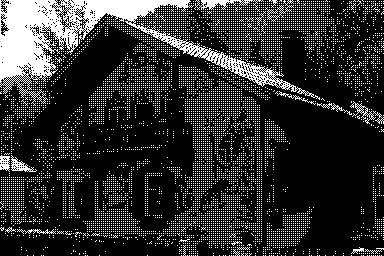
\includegraphics[width=1.0\textwidth]{house_d2.png}
			\caption{Halftoned Image by 2 by 2 Bayer Index Matrix}
		\end{subfigure}
		\begin{subfigure}{0.5\textwidth}
			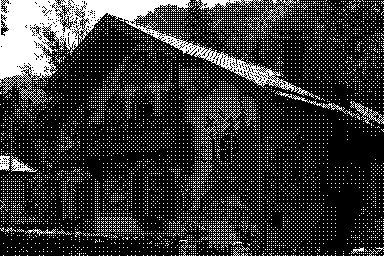
\includegraphics[width=1.0\textwidth]{house_d4.png}
			\caption{Halftoned Image by 4 by 4 Bayer Index Matrix}
		\end{subfigure}
		\begin{subfigure}{1.0\textwidth}
			\begin{center}
				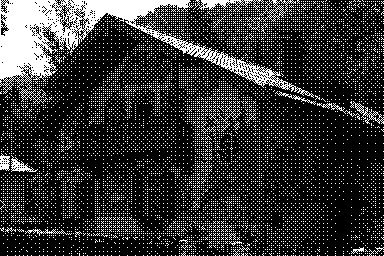
\includegraphics[width=0.5\textwidth]{house_d8.png}
				\caption{Halftoned Image by 8 by 8 Bayer Index Matrix}
			\end{center}
		\end{subfigure}
		\caption{Halftoned Image by Dither Patterns}
	\end{figure}

\subsection{Compute RMSE and Fidelity Values}
	\begin{align*}
		RMSE_{22} &= 97.6690 \\
		fidelity_{22} &= 50.0569
	\end{align*}
	\begin{align*}
		RMSE_{44} &= 101.0069 \\
		fidelity_{44} &= 16.5583
	\end{align*}
	\begin{align*}
		RMSE_{88} &= 100.9145 \\
		fidelity_{88} &= 14.6918
	\end{align*}

%----------------------------------------------------------------------------------------
%	SECTION 5
%----------------------------------------------------------------------------------------

\section{Error Diffusion}

\subsection{Code listing}
	\subsubsection{errDiffusion.m}
	\inputminted[tabsize=2]{matlab}{../source/errDiffusion.m}
	\subsubsection{sec51.m}
	\inputminted[tabsize=2]{matlab}{../source/sec51.m}

\subsection{Original Image vs. Error Diffused Image}
	\begin{figure}[h]
		\begin{subfigure}{0.5\textwidth}
			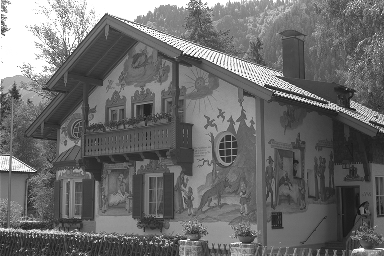
\includegraphics[width=0.9\textwidth]{house.png}
			\caption{Original house.tif}
		\end{subfigure}
		\begin{subfigure}{0.5\textwidth}
			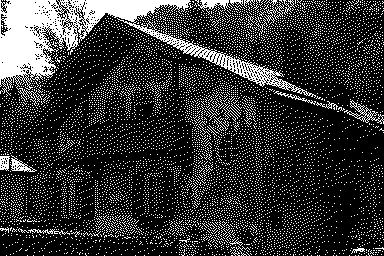
\includegraphics[width=0.9\textwidth]{house_ed.png}
			\caption{Error Diffusion Image}
		\end{subfigure}
		\caption{Orignal and Error Diffusion Image}
	\end{figure}

\subsection{Compute RMSE and Fidelity Values}
	\begin{align*}
		RMSE &= 98.8471 \\
		fidelity &= 13.4273
	\end{align*}

\subsection{RMSE and Fidelity Comparison}
	\begin{table}[h!]
		\begin{center}
			\begin{tabular}{| c | c | c | c | c | c |}
			\hline
				& Threshold & 2x2 Dithering & 4x4 Dithering & 8x8 Dithering
				& Error Diffusion \\ \hline
				RMSE & 87.3933 & 97.6690 & 101.0069 & 100.9145 & 98.8471 \\ \hline
				Fidelity & 77.3371 & 50.0569 & 16.5583 & 14.6918 & 13.4273 \\ \hline
			\end{tabular}
			\caption{RMSE and Fidelity Comparison Table}
			\label{table:1}
		\end{center}
	\end{table}

	Observation: it is clear from the table that the RMSE does not change
	significantly for different methods. However, fidelity does change and it can
	be observed that the threshold method has the highest fidelity value which is
	counter-intuitive since visually speaking, it's the worst.

\end{document}
